\documentclass[lineno]{jfm}

\usepackage{graphicx}
%\usepackage{epstopdf,epsfig}
\usepackage{newtxtext}
\usepackage{newtxmath}
\usepackage{natbib}
\usepackage{hyperref}
\hypersetup{
    colorlinks = true,
    urlcolor   = blue,
    citecolor  = black,
}
\newtheorem{lemma}{Lemma}
\newtheorem{corollary}{Corollary}
\newcommand{\RomanNumeralCaps}[1]
\linenumbers


% {\MakeUppercase{\romannumeral #1}}

\title{Turbulent flow in porous media}

\author{Florencia Falkinhoff\aff{1}
  \corresp{\email{florencia.falkinhoff@ens-lyon.fr}},
  Alexandre Ponomarenko\aff{1}, Mica\aff{1}, Romain Volk\aff{1}, Jean-Lou Pierson\aff{2}
 \and Lionel Gamet\aff{2}}

\affiliation{\aff{1}LPENS
\aff{2}IFPEN}


\begin{document}
\maketitle

\begin{abstract}
Notes about the experiment Darcy02. The experiment, the problems, the results.
\end{abstract}

\begin{keywords}
Authors should not enter keywords on the manuscript, as these must be chosen by the author during the online submission process and will then be added during the typesetting process (see \href{https://www.cambridge.org/core/journals/journal-of-fluid-mechanics/information/list-of-keywords}{Keyword PDF} for the full list).  Other classifications will be added at the same time.
\end{keywords}

{\bf MSC Codes }  {\it(Optional)} Please enter your MSC Codes here


\section{How to submit to the \emph{Journal of Fluid Mechanics}}
\label{sec:intro}

 Authors must submit using the online submission and peer review system \href{https://mc.manuscriptcentral.com/jfm} {Scholar One} (formerly Manuscript Central). If visiting the site for the first time, users must create a new account by clicking on 

\begin{figure}
  \centerline{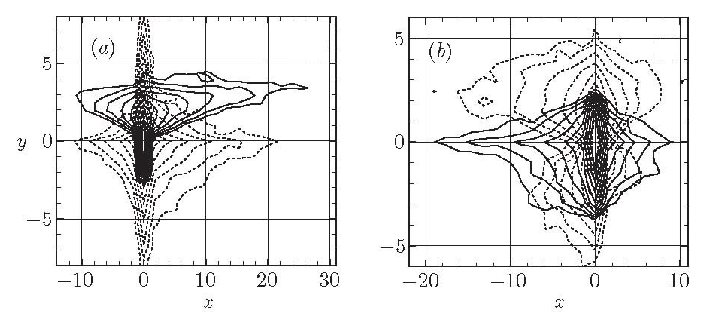
\includegraphics{Fig1}}% Images in 100% size
  \caption{Trapped-mode wavenumbers, $kd$, plotted against $a/d$ for
    three ellipses:\protect\\
    ---$\!$---,
    $b/a=1$; $\cdots$\,$\cdots$, $b/a=1.5$.}
\label{fig:ka}
\end{figure}

\section{How to submit to the \emph{Journal of Fluid Mechanics}}
\label{sec:intro}

 Authors mu

\section{Details for the experiement shown in the abstract}

frames per second: $780$fps.\\
exposure time: $1282$  $\mu$s\\



\section{Introduction}
introduction introduction introduction

\subsection{Discussion Vincent}

fraction volumique tas de billes molles.?

\begin{figure}
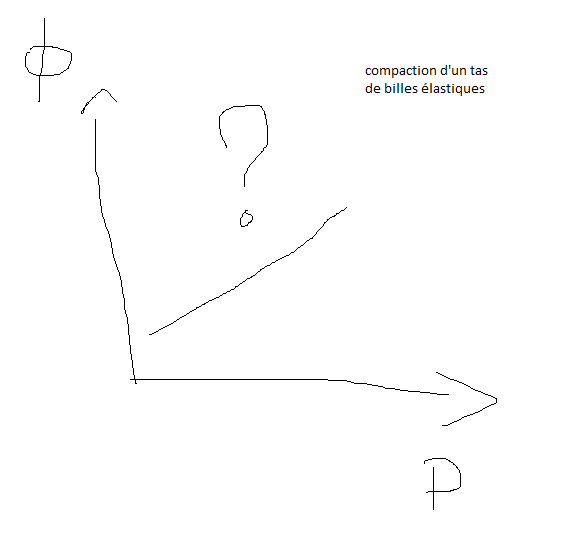
\includegraphics[height=8cm]{figures/elasticBeadsStack_VolumicFraction.png}
\caption{Figure idea about the volumic fraction of an elastic stack of beads.}
\label{fig:volFrac_elasticStac}
\end{figure}

\subsection{Notes pour discussion avec Romain Volk}

\begin{itemize}
    \item achat billes pour remplir la colonne.
    \item Analyse 3D.
    \item Analyse PTV.
    \item Qualité caméra VS qualité téléphone portable?
\end{itemize}


\begin{figure}
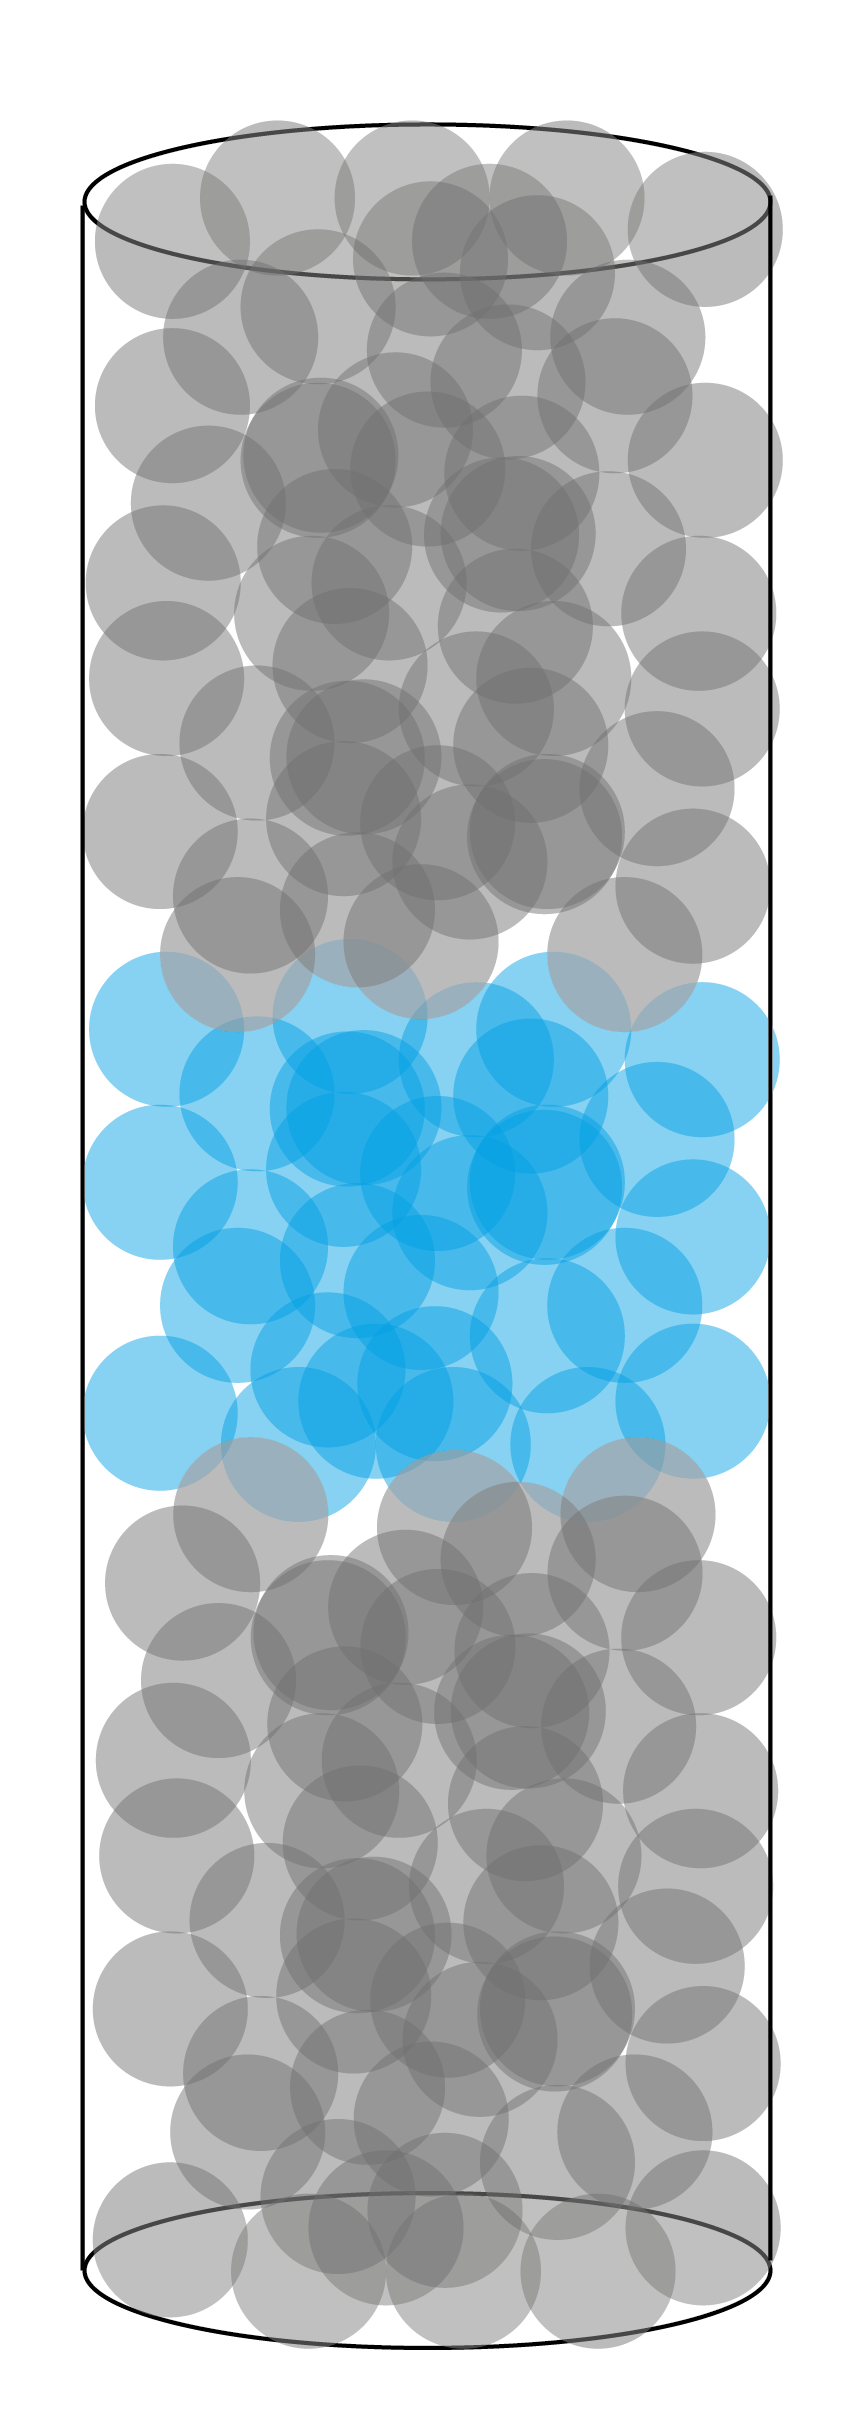
\includegraphics[height=8cm]{figures/beadsStack.png}
\caption{beads}
\label{fig:beads}
\end{figure}

%\begin{figure}
%\includegraphics[width=8cm]{figures/SEM-1.eps}\vspace{-2.2cm}\hspace{-3.2cm}
%\includegraphics[width=3cm]{./makefig0/SEM/SEM-2.eps}\vspace{2.2cm}\\
%\caption{}
%\end{figure}

% * <fulton.rockwell@gmail.com> 2017-05-29T12:21:57.317Z:
% 
% Do we need to invoke capillary sealing here? Or can we just note that at some critical pressure air can invade across the membrane?
% 
% ^.
\begin{equation}
p^{*}\approx \frac{2\gamma}{r^{*}}.\label{eq:ppit}
\end{equation}

\section{TODO list}

- gcc compilateur c++
- mpi for parallelisation

\subsection{Calibration with two level target}

Adapt David Dumond 4DPTV program to the new scale target.\\

Remarks: for the calculation of the spatial transformation from image points (pimg) to 2D postition in real space (pos2D), the code uses the function $T3rw2px  = fitgeotrans(pimg,pos2D,'polynomial',3);$, if there is not enough points it reports : " Error using images.geotrans.PolynomialTransformation2D (line 162)
At least 10 non-collinear points needed to infer polynomial transform. " . To deal with that, a possibility is to set the polynomial degree to $2$ instead of $3$.\\

Depending on the face you look at, the square is on a up line or on a down line. On figure (\ref{fig:caltarget}), the square is on an UP line.

The calibration target has $23$ lines. The DOWN lines have $12$ circles. The UP lines have 11 circles. There are two aditional elements: a square on line $11$ and a triangle on line $12$. There is a total of $143$ circles on DOWN lines and $121$ circles on UP lines plus a square on line $11$ and a triangle on line $12$. \\

Workflow for doing the calibration with this special target: 

\begin{figure}
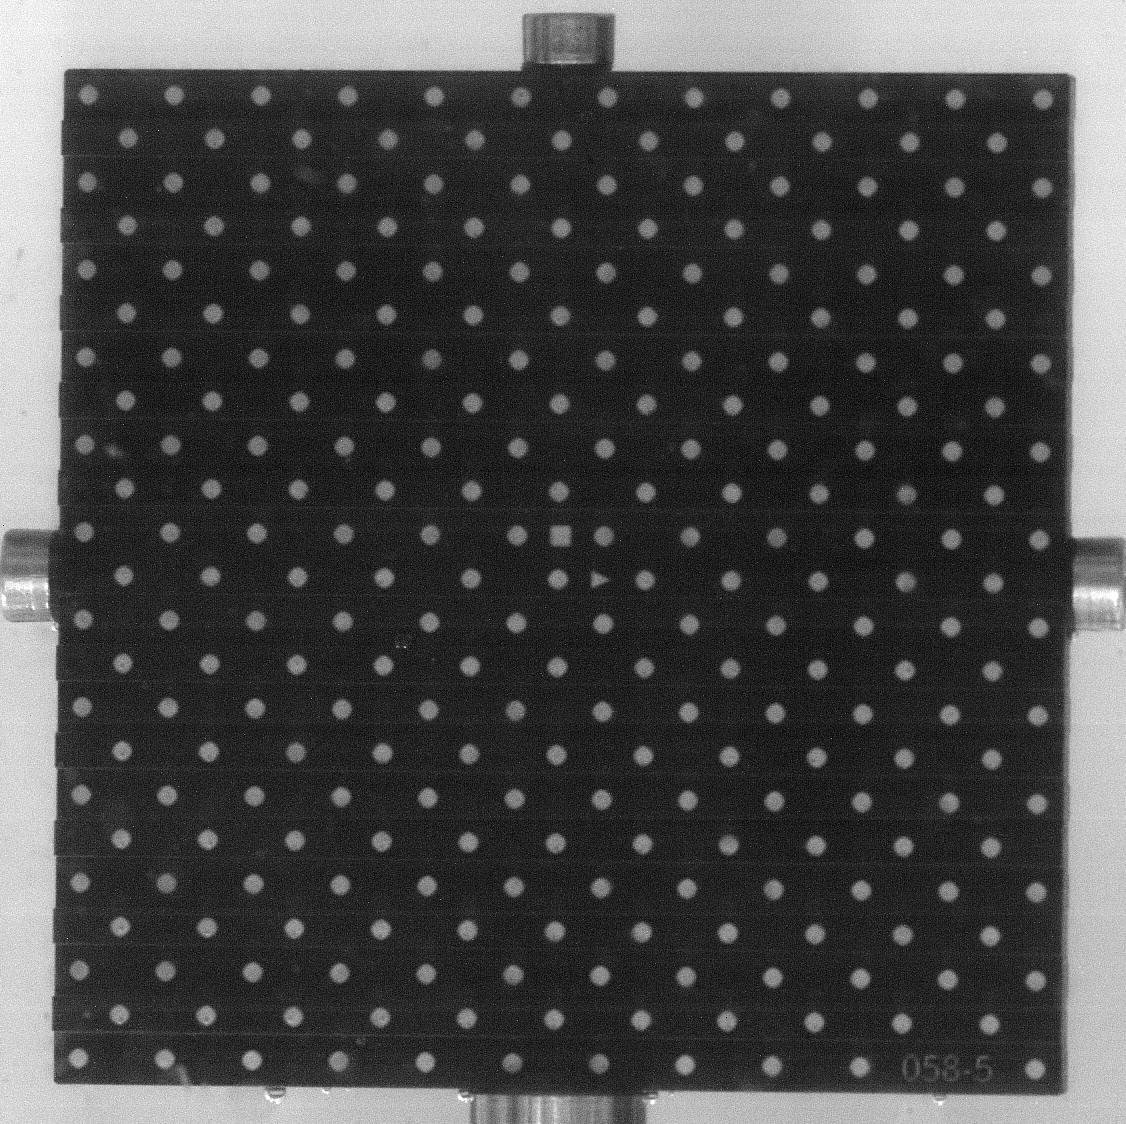
\includegraphics[height=8cm]{figures/calibrationTarget.png}
\caption{calibration target}
\label{fig:caltarget}
\end{figure}


%%%%%%%%%%%%%%%%%%%%%%%%%%%%%%%%%%%%%%%%%%%%
%%%%%%%%%%%%%%%%%%%%%%%%%%%%%%%%%%%%%%%%%%%%
%%%%%%%%%%%%%%%%%%%%%%%%%%%%%%%%%%%%%%%%%%%%
\section{Material and Methods}

\subsection{4D PTV}

The code is on github \href{https://github.com/turbulencelyon/4d-ptv}{4D-ptv on git} and the documentation on \href{https://4d-ptv.readthedocs.io/en/latest/}{read the docs}. 


I install VisualStudioCode, and add C++ tools following this tutorial \href{https://code.visualstudio.com/docs/languages/cpp}{Visual Studio Code C++}. I can compile C++ code.

Installing gcc. I used tips from here: \href{https://www.cs.odu.edu/~zeil/cs250PreTest/latest/Public/installingACompiler/}{link} but I downloaded MinGCW from \href{https://sourceforge.net/projects/mingw-w64/files/Toolchains\%20targetting\%20Win32/Personal\%20Builds/mingw-builds/installer/mingw-w64-install.exe/download}{download MinGW} as indicated on VSCode infos: \href{https://code.visualstudio.com/docs/cpp/config-mingw}{VSCode MinGW}

Change drive in command prompt. To go to D: cd /d D:
Instead of 'make', use 'mingw32-make'

Install hf5++ , good guide \href{https://accserv.lepp.cornell.edu/svn/packages/hdf5/release_docs/INSTALL}{here} and maybe also \href{http://hdf-forum.184993.n3.nabble.com/Trouble-compiling-with-h5c-td4027367.html}{here} and \href{https://stackoverflow.com/questions/60271865/compiling-hdf5-source-with-g}{here}

\subsubsection{PSMN}

./STM -i "./test/rays.dat" -o "./test/" -f 10 -c 2 -d 0.2 -s 1 -m 2 -x 400 -y 400 -z 400 -b -3 3 -3 3 1 5 --hdf5 >> rays.log


\subsection{Sketch plugging the two cameras together}

Shut off all Windows fire walls\\
terminal:\\
ping 100.100.111.52\\
ping 100.100.118.227\\

\subsection{index matching beads}
\subsubsection{Hydrogel beads}
There are three hydrogel beads names $1$, $2$ and $3$.
Order of preference: $1$, $3$, $2$.

About hydrogel beads $2$. They come in pinky pockets named Jelly-Beads, containing $5.1$g of beads that means $\sim300$ beads
\subsection{Flow Meter}

\subsection{solenoid valve: Burkert}

\subsection{tunings for electrovannes}

note from 2021 01 15\\
electrovanne\\
ancien réglage (DARCY 01):\\
low  564 \\
high 665\\


\subsection{3D printer}

\subsection{HDR image from bracketing exposure time image sequence}


\href{https://docs.opencv.org/master/d3/db7/tutorial_hdr_imaging.html}{open CV}


\href{https://towardsdatascience.com/hdr-imaging-what-is-an-hdr-image-anyway-bdf05985492c}{hdr}

\href{https://www.dpreview.com/articles/9828658229/computational-photography-part-i-what-is-computational-photography/2}{dp review}

\subsection{bracketing time lapse}

List of links to took pictures with the camera:
Digicam control command lines: \href{http://digicamcontrol.com/doc/userguide/cmd }{digicam command line}
Info taken from here\\ \href{https://stackoverflow.com/questions/43358257/using-digicamcontrol-to-control-nikon-camera-using-python}{digicam control and python} \\ 
and here \\
\href{http://www.pauldebevec.com/Research/HDR/}{HDR}  \\
and here\\
\href{https://fr.mathworks.com/matlabcentral/fileexchange/57196-cameracontroller?s_tid=FX_rc3_behav}{mathworks file exchange} \\

Some information for processing .NEF pictures:
A comibnation of matrawread (from \href{https://github.com/QiuJueqin/MatRaw}{git hub mat raw}) and dcraw.exe from \href{https://www.dechifro.org/dcraw/}{dcraw}
$\&$ \href{https://www.fastpictureviewer.com/downloads/#links}{soft from a website}

Use of dcraw: \href{https://www.programmersought.com/article/46784093292/}{dcraw}

\href{https://www.cnba.it/contenuti/uploads/2016/03/Processing-RAW-Images-in-MATLAB-Sumner.pdf}{matlab and raw}

finally, dcraw.exe got here: \href{https://fr.osdn.net/projects/sfnet_dcrawnet/downloads/dcraw.exe/}{download dcraw}

From image analysis boss from matlab:
\href{https://blogs.mathworks.com/steve/2011/03/08/tips-for-reading-a-camera-raw-file-into-matlab/}{matlab tips}


\subsubsection{HDR from serie of .NEF}

\noindent \href{https://pypi.org/project/rawhdr/}{link 01}\\
\noindent \href{https://github.com/fthaler/rawhdr}{link 02}\\
\noindent \href{https://learnopencv.com/high-dynamic-range-hdr-imaging-using-opencv-cpp-python/}{link 03}\\
\noindent \href{https://stackoverflow.com/questions/30010227/how-could-i-get-the-raw-pixel-data-out-of-a-nef-file-using-python}{link 04}\\


\subsection{mirrorless ?}

\href{https://www.dxomark.com/things-are-heating-up-in-the-full-frame-mirrorless-camera-market/}{dxoMark}

\href{https://www.jmpeltier.com/disadvantages-of-mirrorless-cameras/}{mirror less is bad}

not happy with a7: \href{https://fstoppers.com/originals/i-wish-id-known-i-moved-sony-366521}{a7 is bad}


\subsection{negative shutter time on cameras ?}
\href{https://photodoto.com/here-is-why-mirrorless-cameras-have-shutters/



\section{list of the experiments}

\subsection{experiment 2021 05 28}

We make a calibration in air.\\
We record an image sequence at $50$Hz of a black point drawn on a white paper which is moved in $3$D. The dot position in 2D on each camera is tracked with FIJI (smooth $\rightarrow$ threshold $\rightarrow$ analyse particles). The IMAGEJ points are saved in Matlab variables 'Camera0\_FIJI' and 'Camera1\_FIJI'. \\
Then rays are crossed and it gives points in 3D. As seen on the figures.

\section{Preliminary results}




%\bibliographystyle{jfm}
%\bibliography{jfm}
%Use of the above commands will create a bibliography using the .bib file. Shown below is a bibliography built from individual items.

\bibliographystyle{jfm}
%\bibliography{jfm2esam}

\begin{thebibliography}{99}

\expandafter\ifx\csname natexlab\endcsname\relax
\def\natexlab#1{#1}\fi
\expandafter\ifx\csname selectlanguage\endcsname\relax
\def\selectlanguage#1{\relax}\fi

\bibitem[Batchelor (1971)]{Batchelor59}
{\sc Batchelor, G.K.} 1971 {Small-scale variation of convected quantities like temperature in turbulent fluid part1, general discussion and the case of small conductivity}, {\it J. Fluid Mech.}, {\bf 5}, pp. 3-113-133.

\bibitem [Bouguet (2008)]{Bouguet01}
{\sc Bouguet, J.-Y} 2008 Camera Calibration Toolbox for Matlab {\url{http://www.vision.caltech.edu/bouguetj/calib_doc/}}.

 \bibitem[Briukhanovetal et al (1967)] {Briukhanovetal1967}
{\sc Briukhanov, A. V.,   Grigorian, S. S., Miagkov,  S. M., Plam, M. Y.,   I. E. Shurova, I. E.,   Eglit, M. E. and Yakimov, Y. L.} 1967
{On some new approaches to the dynamics of snow avalanches},
{\it Physics of Snow and Ice,  Proceedings of the International Conference on Low Temperature Science}
{Vol 1} pp. 1221--1241 {Institute of Low Temperature Science, Hokkaido University, Sapporo, Hokkaido, Japan}.

\bibitem[Brownell (2004)]{Brownell04}
 {\sc Brownell,  C.J.  and Su,  L.K.} 2004  {Planar measurements of differential diffusion in turbulent jets}, {\it AIAA Paper},  pp. 2004-2335.

\bibitem[Brownell and Su (2007)] {Brownell07}
  {\sc Brownell, C.J. and  Su, L.K.} 2007 {Scale relations and spatial spectra in a differentially diffusing jet}, {\it AIAA Paper}, pp 2007-1314.

\bibitem [Dennis (1985)] {Dennis85}
 {\sc  Dennis, S.C.R.} 1985 {Compact explicit finite difference approximations to the Navier--Stokes equation},  { In \it Ninth Intl Conf. on Numerical Methods in Fluid Dynamics},  {ed Soubbaramayer and J.P. Boujot},  {Vol 218}, {\it Lecture Notes in Physics}, pp. 23-51. Springer.

\bibitem [Edwards et al. (2017)]{EdwardsVirouletKokelaarGray2017}
{\sc Edwards, A. N., Viroulet, S., Kokelaar, B. P. and Gray, J. M. N. T.} 2017 Formation of levees, troughs and elevated channels by avalanches on erodible slopes {\it J. Fluid Mech.}, {\bf 823}, pp. 278-315.

\bibitem[Hwang et al (1970)] {Hwang70}
 {\sc Hwang,  L.-S.  and  Tuck, E.O.} 1970 On the oscillations of harbours of arbitrary shape {\it J.~Fluid Mech.}, {\bf42}, pp 447-464.

\bibitem[Josep and Saut (1990)] {JosephSaut1990}
 {\sc Joseph, Daniel D. and Saut, Jean Claude} 1990 Short-wave instabilities and ill-posed initial-value problems {\it Theoretical and Computational Fluid Dynamics}, {\bf 1},  pp.191--227,  {\url{http://dx.doi.org/10.1007/BF00418002}}.

\bibitem[Worster (1992)] {Worster92}
{ \sc  Worster, M.G.} 1992 The dynamics of mushy layers {\it Interactive dynamics of convection and solidification},
{(ed. S.H. Davis and H.E. Huppert and W. Muller and M.G. Worster)}, pp. 113--138 {Kluwer}.

\bibitem[Koch(1983)] {Koch83}
{\sc Koch, W.} 1983 Resonant acoustic frequencies of flat plate cascades {\it J.~Sound Vib.}, {\bf 88}, pp. 233-242.

\bibitem[Lee(1971)] {Lee71}
{\sc Lee,  J.-J.}  1971 Wave-induced oscillations in harbours of arbitrary geometry {\it J.~Fluid Mech.}, {\bf 45}, pp. 375-394.

\bibitem[Linton and  Evans (1992)] {Linton92}
 {\sc  Linton, C.M. and  Evans, D.V.} 1992 The radiation and scattering of surface waves by a vertical circular cylinder in a channel {\it Phil.\ Trans.\ R. Soc.\ Lond.}, {\bf 338}, pp. 325-357.

\bibitem [Martin(1980] {Martin80}
 {\sc  Martin, P.A.} 1980 On the null-field equations for the exterior problems of acoustics {\it Q.~J. Mech.\ Appl.\ Maths},{\bf 33}, pp. 385--396.

\bibitem [Rogallo(1981)] {Rogallo81}
 {\sc Rogallo,  R.S.} 1981 Numerical experiments in homogeneous turbulence  { {\it Tech. Rep.} 81835}  {NASA Tech.\ Mem}.

\bibitem[Ursell(1950)] {Ursell50}
{\sc  Ursell, F.} 1950 Surface waves on deep water in the presence of a submerged cylinder i {\it Proc.\ Camb.\ Phil.\ Soc.}, {\bf 46}, pp.141--152.

\bibitem[Wijngaarden (1968)]{Wijngaarden68}
{\sc van Wijngaarden, L.} 1968 On the oscillations Near and at resonance in open pipes {\it J.~Engng Maths},{\bf 2}, pp. 225--240.

\bibitem[Miller (1991)]{Miller91}
{ \sc  Miller, P.L.} 1991 Mixing in high Schmidt number turbulent jets {school {PhD thesis}} {California Institute of Technology}.

\end{thebibliography}

%% End of file `jfm2esam.bib'.

\end{document}
